\documentclass[11pt]{article}

\usepackage[margin=1in]{geometry}
\usepackage[T1]{fontenc}
\usepackage[utf8]{inputenc}
\usepackage{lmodern}
\usepackage{microtype}
\usepackage{booktabs}
\usepackage{tabularx}
\usepackage{array}
\usepackage{xcolor}
\usepackage{hyperref}
\usepackage{enumitem}
\usepackage{tikz}
\usepackage{pgfplots}
\usepackage{listings}
\usepackage[numbers,sort&compress]{natbib}

\pgfplotsset{compat=1.18}
\usetikzlibrary{arrows.meta,positioning,fit,shapes.geometric}

\definecolor{mlblue}{HTML}{2F6F73}
\definecolor{mlred}{HTML}{8F4F3F}
\definecolor{mlgold}{HTML}{A98A3F}
\definecolor{mlpaper}{HTML}{F7F4EE}
\lstdefinestyle{metta}{
  basicstyle=\ttfamily\small,
  breaklines=true,
  frame=single,
  columns=fullflexible,
  backgroundcolor=\color{mlpaper},
  rulecolor=\color{mlgold!70}
}

\title{TRM-MCP: Efficient Context with DRAM-trained Retrieval }
\author{Patrick Dugan\\Morality Lab}
\date{May 6, 2026}

\begin{document}
\maketitle

\begin{abstract}
Model Context Protocol (MCP) surfaces expose tools, resources, templates, and structured memory, but a small model can waste most of its active context repeatedly scanning the same lookup surface. We propose TRM-MCP: a decomposition in which Tiny Recursive Models (TRMs) learn where to look, which handle or template to use, whether retrieved evidence is relevant, and when to stop. The current artifact set includes a generic MCP trace matrix across filesystem, GitHub, and Postgres-like surfaces with 15 traces and 42 route/retrieve/verify rows; a Primehub schema-retrieval live study on Qwen3.5-9B; and a storyworld play-diary MCP environment study over 15 scenarios and 20 plays. The Primehub study shows retrieval-assisted schema memory improving exact-structure reward on \texttt{ascii\_tree} from 0.0 to 0.8 and \texttt{pydantic\_adherence} from 0.0 to 1.0, while using more tokens in this implementation. The storyworld study shows average diary lift of +0.619333 and recovery from four negative-NAV cases. These results motivate a concrete research program: train small controllers to emit retrieval pointers and stop/escalate decisions over structured external memory, optimizing capability per token rather than raw generation alone.
\end{abstract}

\section{Thesis}

Model Context Protocols (MCPs) had limited early success due to the token-cost of a model reasoning about where and how to retrieve data, the chain-of-thought tokens could be cleared once the curated context was assembled from database queries, but at economic cost. Our central claim is that MCP should be treated as an addressable memory surface for training Tiny Recursive Models (TRMs) to do the retrieval for the LLM. A TRM does not need to know the contents of the filesystem, repository, database, log history, or world model index. It needs to learn a compact policy:

\begin{enumerate}[leftmargin=*]
  \item Which MCP family should be queried?
  \item Which URI, template, entity, or handle is likely relevant?
  \item Is the selected resource an exact hit, a near miss, wrong scope, or wrong family?
  \item Has enough evidence been retrieved?
  \item Should the system stop, continue, or escalate?
\end{enumerate}

This makes TRM-MCP a control-plane architecture rather than a knowledge-distillation architecture. The TRM outputs pointers and actions, not prose answers. The language model remains useful for synthesis, but exact lookup and verification are shifted into typed, trainable control surfaces.

This decomposition follows the same compactification logic as HRM and TRM-style recursive reasoning models \citep{wang2025hrm,jolicoeurmartineau2025trm}, but applies it to context access rather than puzzle solving alone. MeTTa and OpenCog Hyperon motivate the symbolic side of the design: handles, answer shapes, failure modes, and validators can be represented as editable metagraph objects rather than hidden prompt prose \citep{goertzel2021metta,meredith2023metametta}. In the Hermes setting, this connects to tool-use and skill-harness work on instruction-tuned agents \citep{teknium2024hermes3} and verifier-oriented environments such as Prime Intellect's Intellect and Environments Hub work \citep{primeintellect2025intellect3}.

\section{Architecture}

TRM-MCP decomposes lookup into four roles: an Index TRM that compresses resource labels and query cues into family and answer-shape tags; a Router TRM that selects an MCP family and lookup mode; a Retriever TRM that chooses a URI, template, or parameter sketch; and a Verifier TRM that rejects near misses, wrong-scope resources, and wrong-family matches. The deterministic MCP executor remains outside the model. It lists resources, reads resources, expands templates, and enforces token budgets.

\begin{figure}[t]
\centering
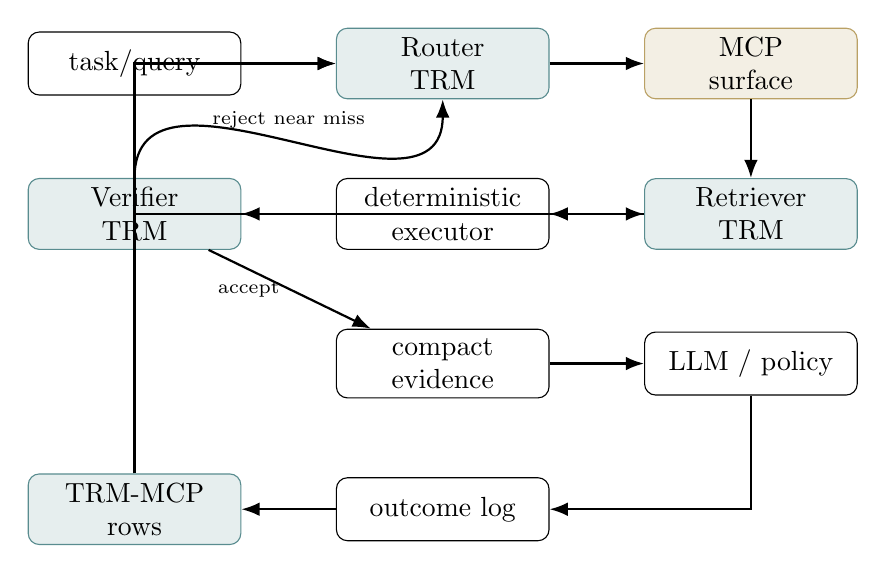
\begin{tikzpicture}[
  node distance=10mm and 12mm,
  box/.style={draw, rounded corners, align=center, minimum width=27mm, minimum height=8mm, fill=white},
  ctrl/.style={box, fill=mlblue!12, draw=mlblue!80},
  mem/.style={box, fill=mlgold!14, draw=mlgold!80},
  arr/.style={-Latex, thick}
]
\node[box] (q) {task/query};
\node[ctrl, right=of q] (router) {Router\\TRM};
\node[mem, right=of router] (mcp) {MCP\\surface};
\node[ctrl, below=of mcp] (retriever) {Retriever\\TRM};
\node[box, left=of retriever] (exec) {deterministic\\executor};
\node[ctrl, left=of exec] (verify) {Verifier\\TRM};
\node[box, below=of exec] (bundle) {compact\\evidence};
\node[box, right=of bundle] (llm) {LLM / policy};
\node[box, below=of bundle] (log) {outcome log};
\node[ctrl, left=of log] (rows) {TRM-MCP\\rows};
\draw[arr] (q) -- (router);
\draw[arr] (router) -- (mcp);
\draw[arr] (mcp) -- (retriever);
\draw[arr] (retriever) -- (exec);
\draw[arr] (exec) -- (verify);
\draw[arr] (verify) -- node[left, font=\scriptsize]{accept} (bundle);
\draw[arr] (verify.north) .. controls +(0,18mm) and +(0,-18mm) .. node[above, font=\scriptsize]{reject near miss} (router.south);
\draw[arr] (bundle) -- (llm);
\draw[arr] (llm) |- (log);
\draw[arr] (log) -- (rows);
\draw[arr] (rows) |- (router);
\draw[arr] (rows) |- (retriever);
\end{tikzpicture}
\caption{TRM-MCP treats the MCP layer as structured external memory. Small controllers emit lookup pointers and verifier decisions; the deterministic executor performs the actual resource access.}
\label{fig:arch}
\end{figure}

\section{Generic MCP Trace Matrix}

The generic example matrix covers three MCP-like surfaces: filesystem, GitHub, and Postgres. Each pack has five traces and fourteen TRM rows. The merged matrix has 15 traces, 42 rows, 15 route rows, 12 retrieve rows, 15 verify rows, 36 exact-positive rows, and 6 negative rows \citep{dugan2026trmmcpmatrix}. These traces exercise exact lookup and hard negatives: semantically attractive resources that should be rejected because the scope, family, or answer shape is wrong.

\begin{table}[t]
\centering
\small
\begin{tabular}{lrrrrrr}
\toprule
Pack & Traces & Rows & Route & Retrieve & Verify & Negatives\\
\midrule
filesystem & 5 & 14 & 5 & 4 & 5 & 2\\
GitHub & 5 & 14 & 5 & 4 & 5 & 2\\
Postgres & 5 & 14 & 5 & 4 & 5 & 2\\
\midrule
merged & 15 & 42 & 15 & 12 & 15 & 6\\
\bottomrule
\end{tabular}
\caption{Generic MCP row matrix used as a training-corpus seed for route/retrieve/verify controllers.}
\label{tab:matrix}
\end{table}

This is a training-corpus seed, not a trained neural TRM result. Its value is schema design: it defines row families, labels, negatives, and action surfaces for evaluating retrieval controllers.

\section{DB Lookup Efficiency Model}

The Postgres worked example motivates an analytical efficiency model for typed lookup. For exact schema reads, the naive workflow is modeled as: list schema groups, list candidate relations, then read the selected relation. The TRM-MCP workflow is modeled as: route directly to the expected resource handle and read it. This reduces modeled MCP calls from 3 to 1 and lookup units from 6 to 2. For query-template reads, modeled MCP calls fall from 3 to 1 and lookup units from 5 to 2.

\begin{figure}[t]
\centering
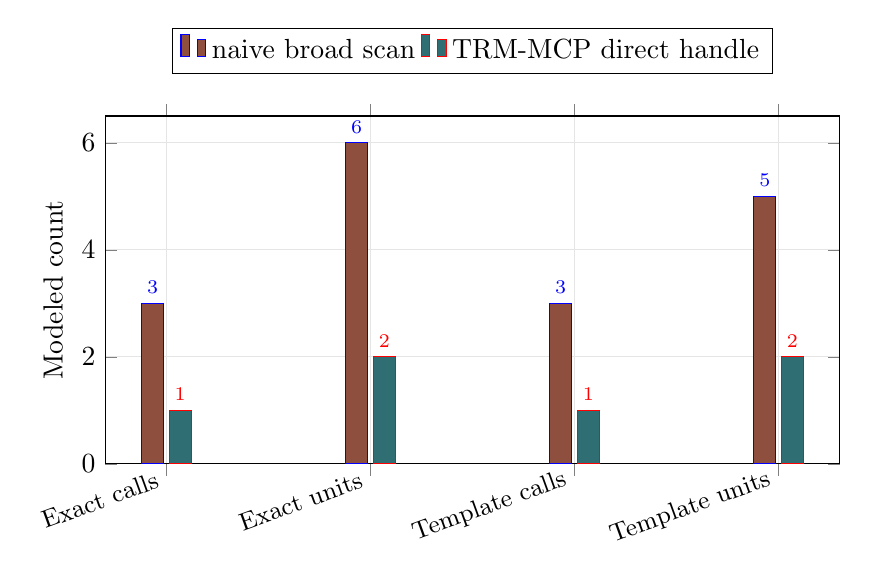
\begin{tikzpicture}
\begin{axis}[
  ybar,
  bar width=8pt,
  width=0.9\linewidth,
  height=6cm,
  ymin=0,
  ymax=6.5,
  ylabel={Modeled count},
  symbolic x coords={Exact calls,Exact units,Template calls,Template units},
  xtick=data,
  x tick label style={font=\small, rotate=20, anchor=east},
  legend style={at={(0.5,1.12)}, anchor=south, legend columns=2},
  nodes near coords,
  nodes near coords style={font=\scriptsize},
  grid=major,
  grid style={draw=gray!20}
]
\addplot+[fill=mlred] coordinates {(Exact calls,3) (Exact units,6) (Template calls,3) (Template units,5)};
\addplot+[fill=mlblue] coordinates {(Exact calls,1) (Exact units,2) (Template calls,1) (Template units,2)};
\legend{naive broad scan, TRM-MCP direct handle}
\end{axis}
\end{tikzpicture}
\caption{Analytical DB lookup model from Postgres trace design. This is not a measured latency or token benchmark; it expresses the intended control-plane advantage of direct handles over broad schema scans.}
\label{fig:dbmodel}
\end{figure}

\section{MeTTa Schema-Surface Enrichment}

A Prime Intellect Environments hub schema MCP pack extends the same idea from SQL-style relation lookup to benchmark schema lookup \citep{dugan2026primehubschema}. A script in the MeTTa programming language defines the MCP schema as a world model to constrain what data trains the retrieval TRMs. The generated surface covers \texttt{psycho\_bench}, \texttt{ascii\_tree}, and \texttt{pydantic\_adherence}. The enriched schema surface contains 6 stable resource handles, 6 answer-shape tags, 6 query-cue sets, 6 minimal examples, 6 failure-mode sets, 2 validation-path or validator-note enriched resources, and 6 source replay links.

The schema surface is produced as a small symbolic contract, not as a long prompt. A representative excerpt of the MeTTa-style atoms used to frame the MCP database surface is:

\begin{lstlisting}[style=metta]
(mcp-surface "primehub_schema")
(resource-handle "primehub_schema" "ascii_tree"
  "mcp://primehub_schema/env/ascii_tree")
(answer-shape "ascii_tree" "ascii_formatted_tree")
(query-cue "ascii_tree" "ASCII tree")
(query-cue "ascii_tree" "<ascii_formatted>")
(failure-mode "ascii_tree" "missing wrapper tags")
(failure-mode "ascii_tree" "extra prose before or after the tree")

(resource-handle "primehub_schema" "pydantic_adherence"
  "mcp://primehub_schema/env/pydantic_adherence")
(answer-shape "pydantic_adherence" "strict_json_object")
(validation-path "pydantic_adherence"
  "extract_last_json -> model_validate_json(strict=False)")
(verifier-note "pydantic_adherence"
  "cooldown accepts integer day counts or numeric strings")
\end{lstlisting}

This is the concrete sense in which MeTTa improves the MCP schema: it turns benchmark prompt fragments, examples, verifier notes, and replay evidence into addressable records that can be routed to, retrieved, and rejected by small controllers.

\begin{figure}[t]
\centering
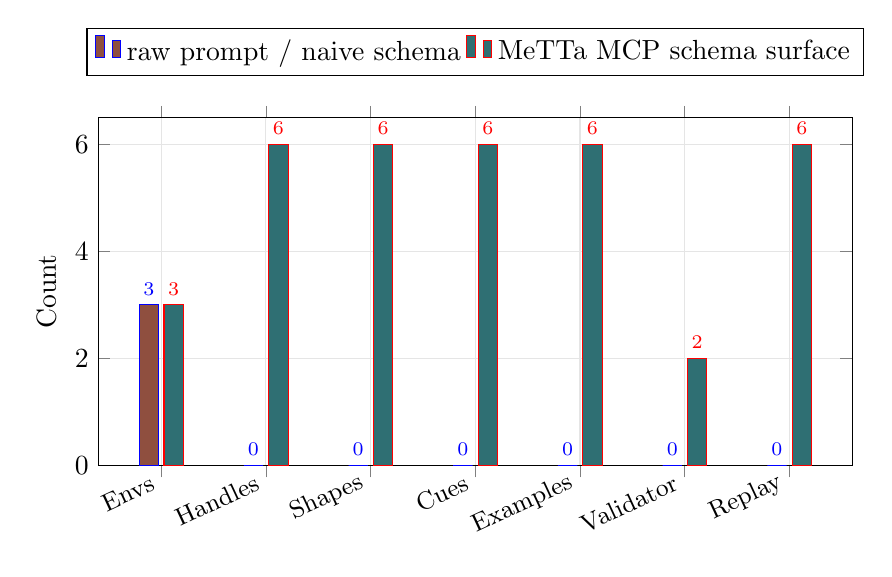
\begin{tikzpicture}
\begin{axis}[
  ybar,
  bar width=7pt,
  width=0.92\linewidth,
  height=6cm,
  ymin=0,
  ymax=6.5,
  ylabel={Count},
  symbolic x coords={Envs,Handles,Shapes,Cues,Examples,Validator,Replay},
  xtick=data,
  x tick label style={font=\small, rotate=25, anchor=east},
  legend style={at={(0.5,1.12)}, anchor=south, legend columns=2},
  nodes near coords,
  nodes near coords style={font=\scriptsize},
  grid=major,
  grid style={draw=gray!20}
]
\addplot+[fill=mlred] coordinates {(Envs,3) (Handles,0) (Shapes,0) (Cues,0) (Examples,0) (Validator,0) (Replay,0)};
\addplot+[fill=mlblue] coordinates {(Envs,3) (Handles,6) (Shapes,6) (Cues,6) (Examples,6) (Validator,2) (Replay,6)};
\legend{raw prompt / naive schema, MeTTa MCP schema surface}
\end{axis}
\end{tikzpicture}
\caption{Schema-surface enrichment from the Primehub schema MCP pack. The current claim is not a live SQL migration; it is that MeTTa/MCP turns vague prompt and replay material into addressable schema records for routing and verification.}
\label{fig:schema}
\end{figure}

\section{Recovered Live Schema-Retrieval Measurement}

The April Primehub structured-map retrieval study contains the primary empirical result for the schema-memory claim \citep{dugan2026primehubretrieval}. The run compares three arms: \texttt{baseline}, with no Hermes structured-map prompt; \texttt{plain\_structured\_map}, with the structured-map skill prompt but no retrieved schema memory; and \texttt{retrieval\_assisted}, with the structured-map prompt plus TRM-MCP-style Primehub schema memory.

\begin{table}[t]
\centering
\small
\begin{tabular}{llrrr}
\toprule
Environment & Arm & Reward & Total tokens & Reward / 1k tokens\\
\midrule
\texttt{ascii\_tree} & baseline & 0.0000 & 497 & 0.0000\\
\texttt{ascii\_tree} & plain & 0.0000 & 656 & 0.0000\\
\texttt{ascii\_tree} & retrieval & 0.8000 & 939 & 0.8520\\
\texttt{psycho\_bench} & baseline & 3.3283 & 1119 & 2.9744\\
\texttt{psycho\_bench} & plain & 3.3061 & 1239 & 2.6684\\
\texttt{psycho\_bench} & retrieval & 3.3311 & 1534 & 2.1715\\
\texttt{pydantic\_adherence} & baseline & 0.0000 & 1243 & 0.0000\\
\texttt{pydantic\_adherence} & plain & 0.0000 & 1364 & 0.0000\\
\texttt{pydantic\_adherence} & retrieval & 1.0000 & 1860 & 0.5376\\
\bottomrule
\end{tabular}
\caption{Recovered live Qwen3.5-9B schema-retrieval measurements. Retrieval-assisted schema memory improves exact-structure reward while using more tokens in this implementation.}
\label{tab:measured}
\end{table}

\begin{figure}[t]
\centering
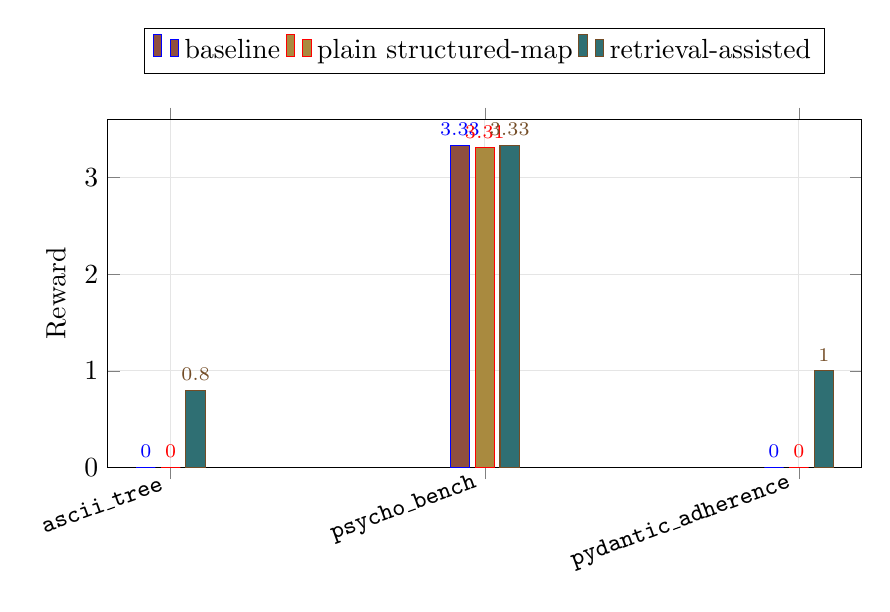
\begin{tikzpicture}
\begin{axis}[
  ybar,
  bar width=7pt,
  width=0.92\linewidth,
  height=6cm,
  ymin=0,
  ymax=3.6,
  ylabel={Reward},
  symbolic x coords={ascii,psycho,pydantic},
  xtick=data,
  xticklabels={\texttt{ascii\_tree},\texttt{psycho\_bench},\texttt{pydantic\_adherence}},
  x tick label style={font=\small, rotate=20, anchor=east},
  legend style={at={(0.5,1.13)}, anchor=south, legend columns=3},
  nodes near coords,
  nodes near coords style={font=\scriptsize},
  grid=major,
  grid style={draw=gray!20}
]
\addplot+[fill=mlred] coordinates {(ascii,0.0) (psycho,3.3283) (pydantic,0.0)};
\addplot+[fill=mlgold] coordinates {(ascii,0.0) (psycho,3.3061) (pydantic,0.0)};
\addplot+[fill=mlblue] coordinates {(ascii,0.8) (psycho,3.3311) (pydantic,1.0)};
\legend{baseline, plain structured-map, retrieval-assisted}
\end{axis}
\end{tikzpicture}
\caption{Measured reward by arm. Retrieval-assisted schema memory unlocks exact structured validity on \texttt{ascii\_tree} and \texttt{pydantic\_adherence}; \texttt{psycho\_bench} was already near-saturated.}
\label{fig:reward}
\end{figure}

\begin{figure}[t]
\centering
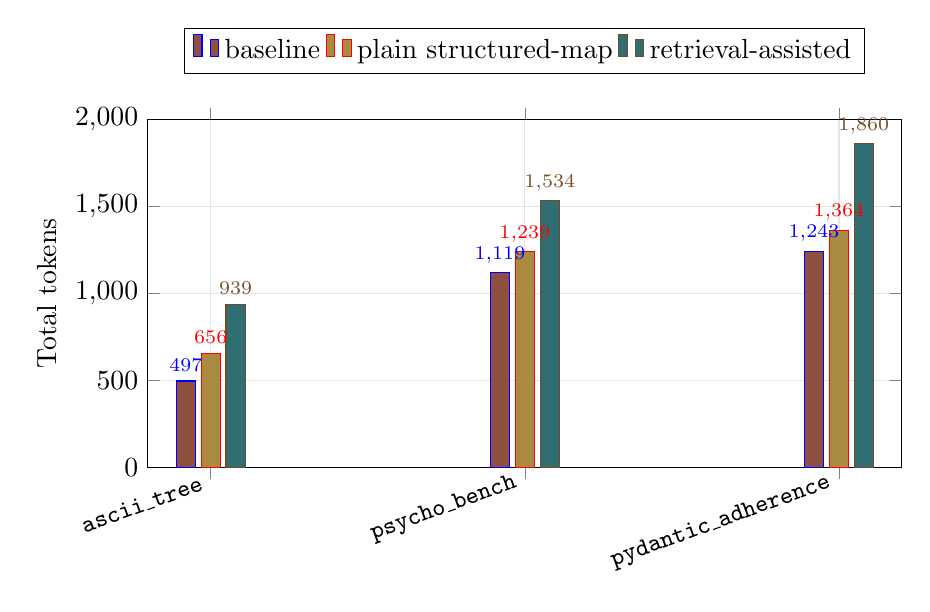
\begin{tikzpicture}
\begin{axis}[
  ybar,
  bar width=7pt,
  width=0.92\linewidth,
  height=6cm,
  ymin=0,
  ymax=2000,
  ylabel={Total tokens},
  symbolic x coords={ascii,psycho,pydantic},
  xtick=data,
  xticklabels={\texttt{ascii\_tree},\texttt{psycho\_bench},\texttt{pydantic\_adherence}},
  x tick label style={font=\small, rotate=20, anchor=east},
  legend style={at={(0.5,1.13)}, anchor=south, legend columns=3},
  nodes near coords,
  nodes near coords style={font=\scriptsize},
  grid=major,
  grid style={draw=gray!20}
]
\addplot+[fill=mlred] coordinates {(ascii,497) (psycho,1119) (pydantic,1243)};
\addplot+[fill=mlgold] coordinates {(ascii,656) (psycho,1239) (pydantic,1364)};
\addplot+[fill=mlblue] coordinates {(ascii,939) (psycho,1534) (pydantic,1860)};
\legend{baseline, plain structured-map, retrieval-assisted}
\end{axis}
\end{tikzpicture}
\caption{Token use by arm. The recovered run does not support a token-reduction claim; retrieval-assisted schema memory spends more tokens but crosses validity thresholds where baseline and plain prompting fail.}
\label{fig:tokens}
\end{figure}

\section{Storyworld Play-Diary MCP}

The storyworld player adds episodic memory. Repeated playthroughs write a diary containing episode summaries, turn rows, legal actions, selected actions, NAV recommendations, endings, scores, and TRM labels. The diary lookup is subordinate to current legal actions: a retrieved action must not be copied unless it appears in the current legal-action set.

The \texttt{overnight\_policy\_v2} run used the \texttt{paper} profile with 15 scenarios, 20 plays, max depth 7, and branch limit 1024 \citep{dugan2026storyworlddiary}. The v2 policy seeds MCP memory with deterministic and NAV rollouts, then lets retrieved outcome evidence override NAV when a remembered legal action has a better score. Average diary lift reached +0.619333. The largest positive lifts were \texttt{market\_square} (+4.4), \texttt{medicine\_dilemma} (+1.4), \texttt{multi\_agent\_release\_council} (+1.64), and \texttt{scarlett\_letter} (+1.85). Four cases where NAV was negative were recovered back to baseline by diary memory.

\begin{figure}[t]
\centering
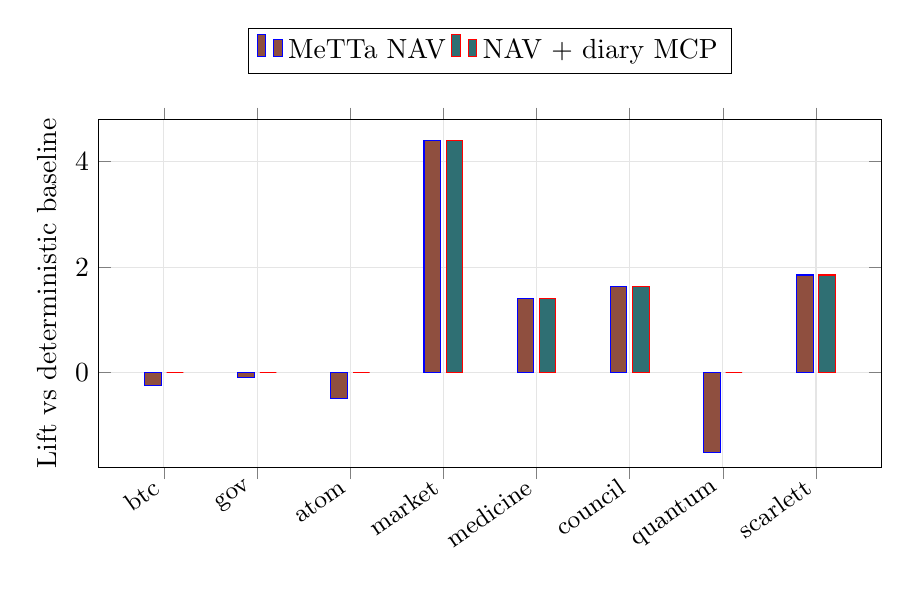
\begin{tikzpicture}
\begin{axis}[
  ybar,
  bar width=6pt,
  width=0.95\linewidth,
  height=6cm,
  ymin=-1.8,
  ymax=4.8,
  ylabel={Lift vs deterministic baseline},
  symbolic x coords={btc,gov,atom,market,medicine,council,quantum,scarlett},
  xtick=data,
  xticklabels={btc,gov,atom,market,medicine,council,quantum,scarlett},
  x tick label style={font=\small, rotate=35, anchor=east},
  legend style={at={(0.5,1.13)}, anchor=south, legend columns=2},
  grid=major,
  grid style={draw=gray!20}
]
\addplot+[fill=mlred] coordinates {(btc,-0.25) (gov,-0.10) (atom,-0.50) (market,4.40) (medicine,1.40) (council,1.64) (quantum,-1.52) (scarlett,1.85)};
\addplot+[fill=mlblue] coordinates {(btc,0.00) (gov,0.00) (atom,0.00) (market,4.40) (medicine,1.40) (council,1.64) (quantum,0.00) (scarlett,1.85)};
\legend{MeTTa NAV, NAV + diary MCP}
\end{axis}
\end{tikzpicture}
\caption{Selected storyworld play-diary MCP lift. Diary memory preserves positive NAV gains and recovers four negative-NAV cases back to baseline.}
\label{fig:diary}
\end{figure}

\section{Training Target}

TRM-MCP training rows should be state-to-retrieval-policy examples, not question-to-answer examples. A minimal row contains task text, compact task state, available MCP families, candidate descriptors, gold route or URI/template, verifier label, retrieved token count, and downstream success or failure. The target should be a structured action such as:

\begin{verbatim}
{
  "family": "storyworld_play_diary",
  "lookup": "turn_history",
  "keys": ["scarlett_letter", "Hester", "MarketScaffold"],
  "top_k": 3,
  "compression": "summary_atoms",
  "decision": "retrieve_then_answer"
}
\end{verbatim}

The most important design choice is pointer output. Natural-language router output wastes tokens and is harder to verify.

\section{Metrics}

Retrieval and downstream metrics should be reported separately: first useful hit rate, MCP calls per task, tokens loaded per task, verifier rejection precision on near misses, solved-task latency, answer or decision quality, quality per 1k retrieved tokens, and catastrophic miss rate. The main scaling metric should be quality-adjusted success per token, not raw success alone.

\section{Limitations}

The generic MCP matrix is currently a curated row set, not a trained neural TRM evaluation. The storyworld diary result is an environment-study result under deterministic/NAV/diary policies. The recovered Primehub schema measurement shows exact-structure validity lift but does not show token savings; retrieval-assisted schema memory used more tokens in that implementation. The Postgres lookup graph is analytical, not a measured latency result. These boundaries are important because the paper's strongest current claim is about structured validity and control-plane decomposition, not universal context-cost reduction.

\section{Conclusion}

TRM-MCP reframes context as a control problem. The immediate evidence does not show that retrieval is automatically cheaper; the recovered Primehub run spends more tokens. It shows something more specific and more useful: when memory is converted into typed handles, answer shapes, examples, failure modes, and verifier notes, small controllers can be trained to retrieve compact evidence rather than asking the language model to repeatedly rediscover the same schema.

This is forward-looking for small models. A compact LLM can remain the prose synthesizer or creative policy, while retrieval, stop/escalate, legality checks, and near-miss rejection move into small trainable modules over MCP memory. The storyworld player MCP used in the Hermes hackathon work is the most concrete version of that idea: repeated play writes diary rows, retrieval brings back relevant outcomes, and current legal actions still gate what the model is allowed to reuse. If this pattern generalizes, small models do not need to become frontier-scale context reasoners to improve; they need reliable typed memory access, cheap verifiers, and controllers trained on the traces of their own failures.

\appendix

\section{Appendix: Router and Verifier TRM Study}

The first follow-on study trains a small router/verifier TRM on the generic matrix plus expanded hard negatives, then evaluates on held-out MCP families. The key metric is not answer prose quality; it is exact family selection, first useful hit, and verifier rejection precision on attractive near misses.

\begin{figure}[h]
\centering
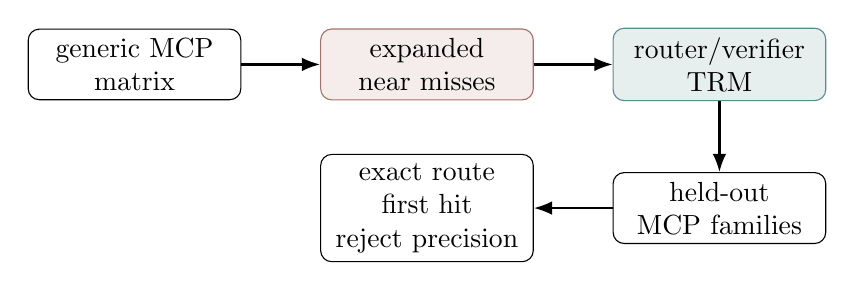
\begin{tikzpicture}[
  node distance=9mm and 10mm,
  box/.style={draw, rounded corners, align=center, minimum width=27mm, minimum height=8mm, fill=white},
  ctrl/.style={box, fill=mlblue!12, draw=mlblue!80},
  neg/.style={box, fill=mlred!10, draw=mlred!80},
  arr/.style={-Latex, thick}
]
\node[box] (matrix) {generic MCP\\matrix};
\node[neg, right=of matrix] (negatives) {expanded\\near misses};
\node[ctrl, right=of negatives] (train) {router/verifier\\TRM};
\node[box, below=of train] (heldout) {held-out\\MCP families};
\node[box, left=of heldout] (metrics) {exact route\\first hit\\reject precision};
\draw[arr] (matrix) -- (negatives);
\draw[arr] (negatives) -- (train);
\draw[arr] (train) -- (heldout);
\draw[arr] (heldout) -- (metrics);
\end{tikzpicture}
\caption{Router/verifier TRM study over held-out MCP families. Expanded negatives test whether the controller rejects plausible but wrong handles before they enter context.}
\label{fig:appendix-router-verifier}
\end{figure}

\section{Appendix: Storyworld Retrieval-TRM}

The second study builds a retrieval-TRM from storyworld play-diary rows and tests repeated play under fixed token budgets. This extends the Hermes hackathon storyworld player MCP: the player accumulates diary rows over playthroughs, retrieves prior outcomes for the current encounter, and only reuses an action if it is legal in the current state.

\begin{figure}[h]
\centering
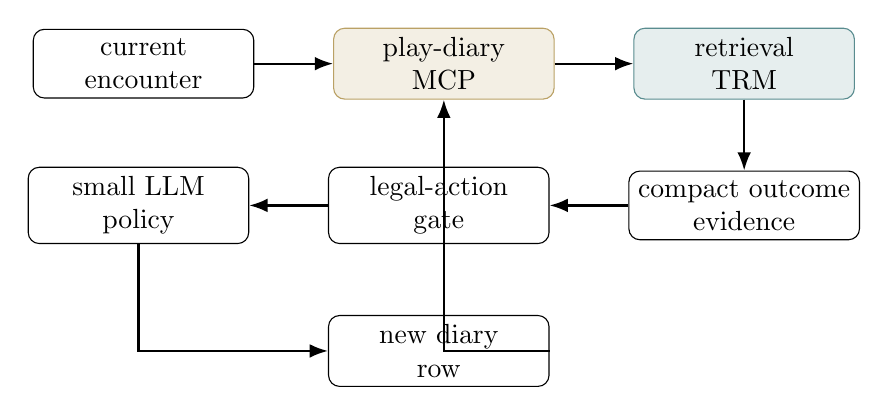
\begin{tikzpicture}[
  node distance=9mm and 10mm,
  box/.style={draw, rounded corners, align=center, minimum width=28mm, minimum height=8mm, fill=white},
  ctrl/.style={box, fill=mlblue!12, draw=mlblue!80},
  mem/.style={box, fill=mlgold!14, draw=mlgold!80},
  arr/.style={-Latex, thick}
]
\node[box] (encounter) {current\\encounter};
\node[mem, right=of encounter] (diary) {play-diary\\MCP};
\node[ctrl, right=of diary] (retriever) {retrieval\\TRM};
\node[box, below=of retriever] (bundle) {compact outcome\\evidence};
\node[box, left=of bundle] (legal) {legal-action\\gate};
\node[box, left=of legal] (policy) {small LLM\\policy};
\node[box, below=of legal] (log) {new diary\\row};
\draw[arr] (encounter) -- (diary);
\draw[arr] (diary) -- (retriever);
\draw[arr] (retriever) -- (bundle);
\draw[arr] (bundle) -- (legal);
\draw[arr] (legal) -- (policy);
\draw[arr] (policy) |- (log);
\draw[arr] (log) -| (diary);
\end{tikzpicture}
\caption{Storyworld retrieval-TRM study. Diary MCP memory improves repeated play only if retrieved outcomes are filtered through current legal actions and score evidence.}
\label{fig:appendix-storyworld-retrieval}
\end{figure}

\section{Appendix: Context-Efficiency Matrix}

The third study compares five context strategies under fixed token budgets: stuffed context, embedding retrieval, rules-only retrieval, TRM-MCP retrieval, and strong-LLM retrieval planners. The outcome should be reported as downstream quality per 1k input tokens, plus catastrophic miss rate and verifier rejection precision.

\begin{figure}[h]
\centering
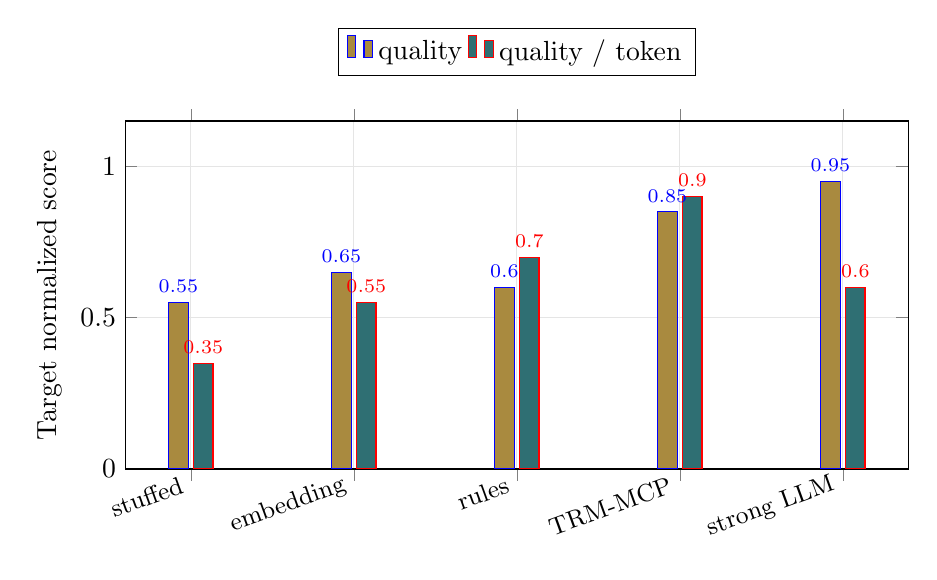
\begin{tikzpicture}
\begin{axis}[
  ybar,
  bar width=7pt,
  width=0.95\linewidth,
  height=6cm,
  ymin=0,
  ymax=1.15,
  ylabel={Target normalized score},
  symbolic x coords={stuffed,embedding,rules,trm-mcp,strong-llm},
  xtick=data,
  xticklabels={stuffed,embedding,rules,TRM-MCP,strong LLM},
  x tick label style={font=\small, rotate=20, anchor=east},
  legend style={at={(0.5,1.13)}, anchor=south, legend columns=2},
  nodes near coords,
  nodes near coords style={font=\scriptsize},
  grid=major,
  grid style={draw=gray!20}
]
\addplot+[fill=mlgold] coordinates {(stuffed,0.55) (embedding,0.65) (rules,0.60) (trm-mcp,0.85) (strong-llm,0.95)};
\addplot+[fill=mlblue] coordinates {(stuffed,0.35) (embedding,0.55) (rules,0.70) (trm-mcp,0.90) (strong-llm,0.60)};
\legend{quality, quality / token}
\end{axis}
\end{tikzpicture}
\caption{Context-efficiency matrix design. Values are placeholders for the follow-on experiment, included to define the reporting shape: quality and quality-per-token should be separated.}
\label{fig:appendix-context-matrix}
\end{figure}

\section*{Artifact Availability}

The bundled CSV files in \texttt{tables/} contain the local values used for the manuscript tables and plots. The principal source artifacts are listed in \texttt{evidence\_manifest.json} in the paper seed directory \citep{dugan2026trmmcpseed}. The current Overleaf package includes source tables and generated figure source, but not the full local replay logs.

\bibliographystyle{plainnat}
\bibliography{references}

\end{document}
